\chapter{Exemplaric Implementation}
\label{chap:implementations}

%////////////////////////////////////////////////
\section{Implementation I: Using Game Engines as Renderers and Frontends}
\subsection{Goals and Constraints of the Implementation}
\label{section:goals-and-constraints}
Inspired by a thesis written by Lucas Schweitzer in 2017 that approached using \acsp{CNN} that detect doors on autonomous robots \cite{Schweitzer2017}, the goal of this thesis' implementation became to generate records that could be used to train \acsp{CNN} that detect doors.\\ 
The environment chosen for this implementation was the second floor of building "A" of University of Applied Sciences Mannheim as this building houses the Faculty of Computer Science and the Institute of Robotics is located in the second floor.\\
This implementation of the concept had the working title "VERE" ("Virtual Environments for Robotics Experiments").

\subsection{Why to Use Game Engines}
Making use of game engines to implement the concept was based on the observation that video games have always striven after improved visual presentation and more intuitive user interaction in order to attract customers, leading to the general availability of game engines that feature impressive graphical detail (as demonstrated in figure \ref{fig:unity-demo-graphics}), intuitive methods to interact with users and great performance on modern computer systems. Their ability to produce realistic images in real-time made them an attractive alternative to traditional offline renderers.
\begin{center}
\noindent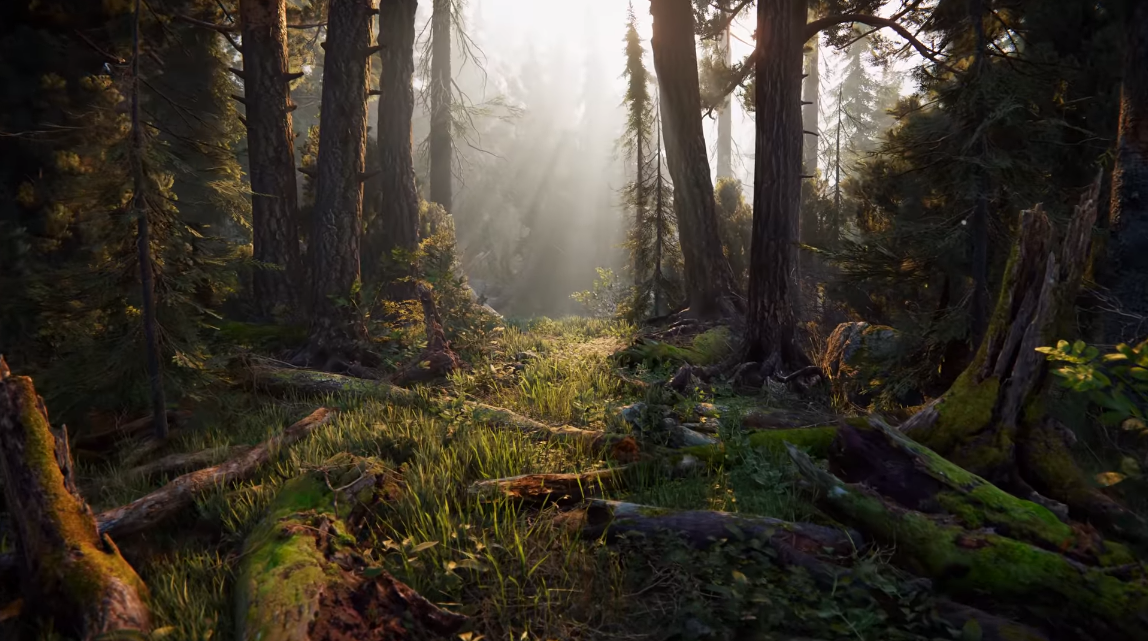
\includegraphics[width=14cm]{tex/img/ch05/UnityGraphicsDemo.png}
\captionof{figure}{Unity Technology's "Book of the Dead" teaser video\cite{UnityDemoRealtimeTeaser}}
\label{fig:unity-demo-graphics}
\end{center}

New rendering-technologies that improve the quality of rendered images and performance of the rendering-process are being developed and published by both proprietary and open-source developers. A current example of a new technology recently published is NVIDIA's proprietary "RTX"-technology \cite{NVIDIARTX} that features "Hybrid Rasterization and Ray Tracing" \cite{NVIDIARayTracing} to combine raytracing and conventional rasterization in the rendering-process. A public demonstration of this new technique was shown running on the "Unreal Engine" in a short video (figure \ref{fig:unreal-demo-graphics})\cite{UnrealDemoReflections}.
\begin{center}
\noindent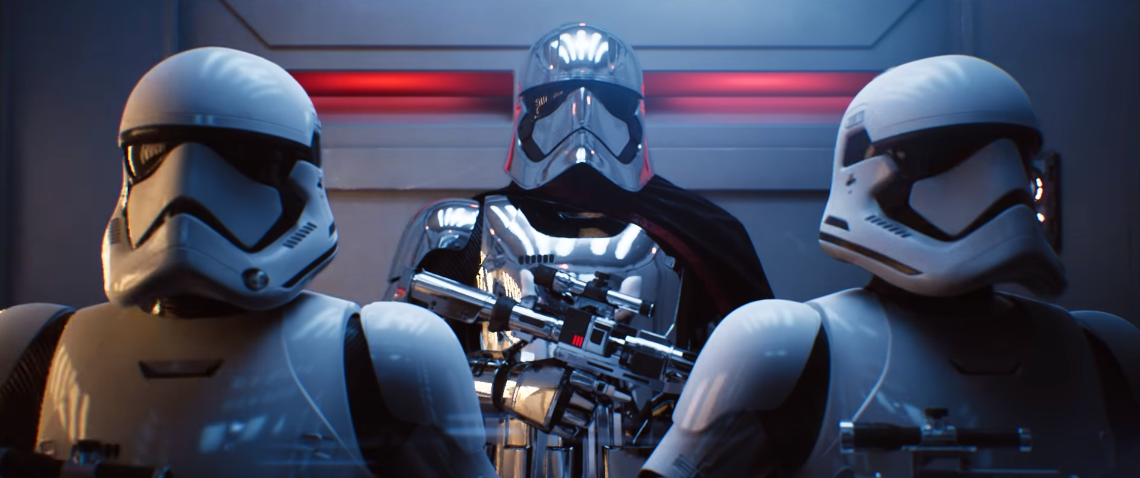
\includegraphics[width=14cm]{tex/img/ch05/UnrealGraphicsDemo.png}
\captionof{figure}{Demonstration of NVIDIA RTX and Microsoft DXR running on the Unreal Engine \cite{UnrealDemoReflections}}
\label{fig:unreal-demo-graphics}
\end{center}

%////////////////////////////////////////////////
\subsubsection{Choosing a Game Engine}
The decision which game engine to use to implement the concept was based on a set of factors that needed to be considered:
\begin{description}
\item [Stability] While the goal of using game engines as real-time renderers is to generate records quickly, recording sessions may take several hours. The software needs to maintain stable operation because recording sessions may run un-supervised and crashes may be detected only hours later.
\item [Crossplatform] Support of multiple platforms serves multiple purposes. First it aims to avoid platform-specific platforms that may either be already existent or yet to come. Operating-system updates can cause software to malfunction as was recently seen with multiple updates of the Windows operating system\cite{heiseWindowsUpdate}. Secondly, supporting multiple platforms greatly extends the potential groups of users. Users that own licenses for proprietary operating systems will be able to run the software on their current systems while users that lack licenses to proprietary operating systems may chose a free operating system. 
\item [Features] As this thesis' concept aims to generate labelled images of excellent quality, the game engine used for rendering said images must feature rendering capabilities that produce realistic output. This requires features like ambient occlusion, anti-aliasing, depth-of-field, high dynamic range rendering and different shading-techniques.
\item [Maintenance] Software is expected to be operable for a certain period. While games may run on modern systems for some years, programming new programs for sophisticated fields of use like research comes at considerable development cost. Therefore one important factor is the expected time a game engine enables software to run on modern systems. One way to evaluate this factor is to study when a game engine was first publicly announced, what games are being published that use the engine and in what intervals it is updated. Dependencies introduced by game engines further add to potential problems with software becoming outdated and unable to use on modern systems. 
\item [Licensing] Like most other software, game engines are usually distributed with licenses that specify under what conditions and for which purposes they may be used. Many engines that power popular games today are exclusive to their developer studios or publishers and are not available for public use (e.g. \textit{Frostbite} that powers the \textit{Battlefield} game-series or \textit{id Tech 6} which \textit{Doom (2016)} was based on). 
\item [Community] When it comes to become acquainted with working a game engine, an active community of developers can prove very useful as documentation may become obsolete when update-cycles of game engines are very short. Open-source projects allow developers to use and learn from others' code so one may be more likely to find open-source projects for popular game engines than less popular ones.
\item [Assets] Some developers of game engines (such as Unity and Unreal Engine) offer access to free or paid assets (such as 3D models, sound and even code) that can be used in projects. Using existing assets saves time during development.
\item [Tools] Popular game engines are usually distributed with tools that streamline the development of games. Some come with feature-rich all-in-one software suites (e.g. Unity, CryEngine and Unreal Engine) that cover tasks like world-building, scripting and compiling. Others provide separate tools like world-editors, conversion-tools or compilers (e.g. Source Engine).
\end{description}

After evaluating modern and popular game engines considering the abovementioned criteria (as shown in \ref{table:game-engines}), the Unity game engine was used for implementation of the concept of this thesis. It was chosen because of its crossplatform-capabilities \cite{UnityPlatformSupport}, regular updates \cite{UnityDownloadArchive}, free use for educational purposes \cite{UnityForEducation}, active community of developers \cite{UnityForum} and built-in editor-application. It features a free post-processing stack \cite{UnityPostProcessingStack} and built-in editor (shown in figure \ref{fig:unity-editor}) that allows developers to build scenes, configure objects in scenes and test run their games.
\begin{center}
\noindent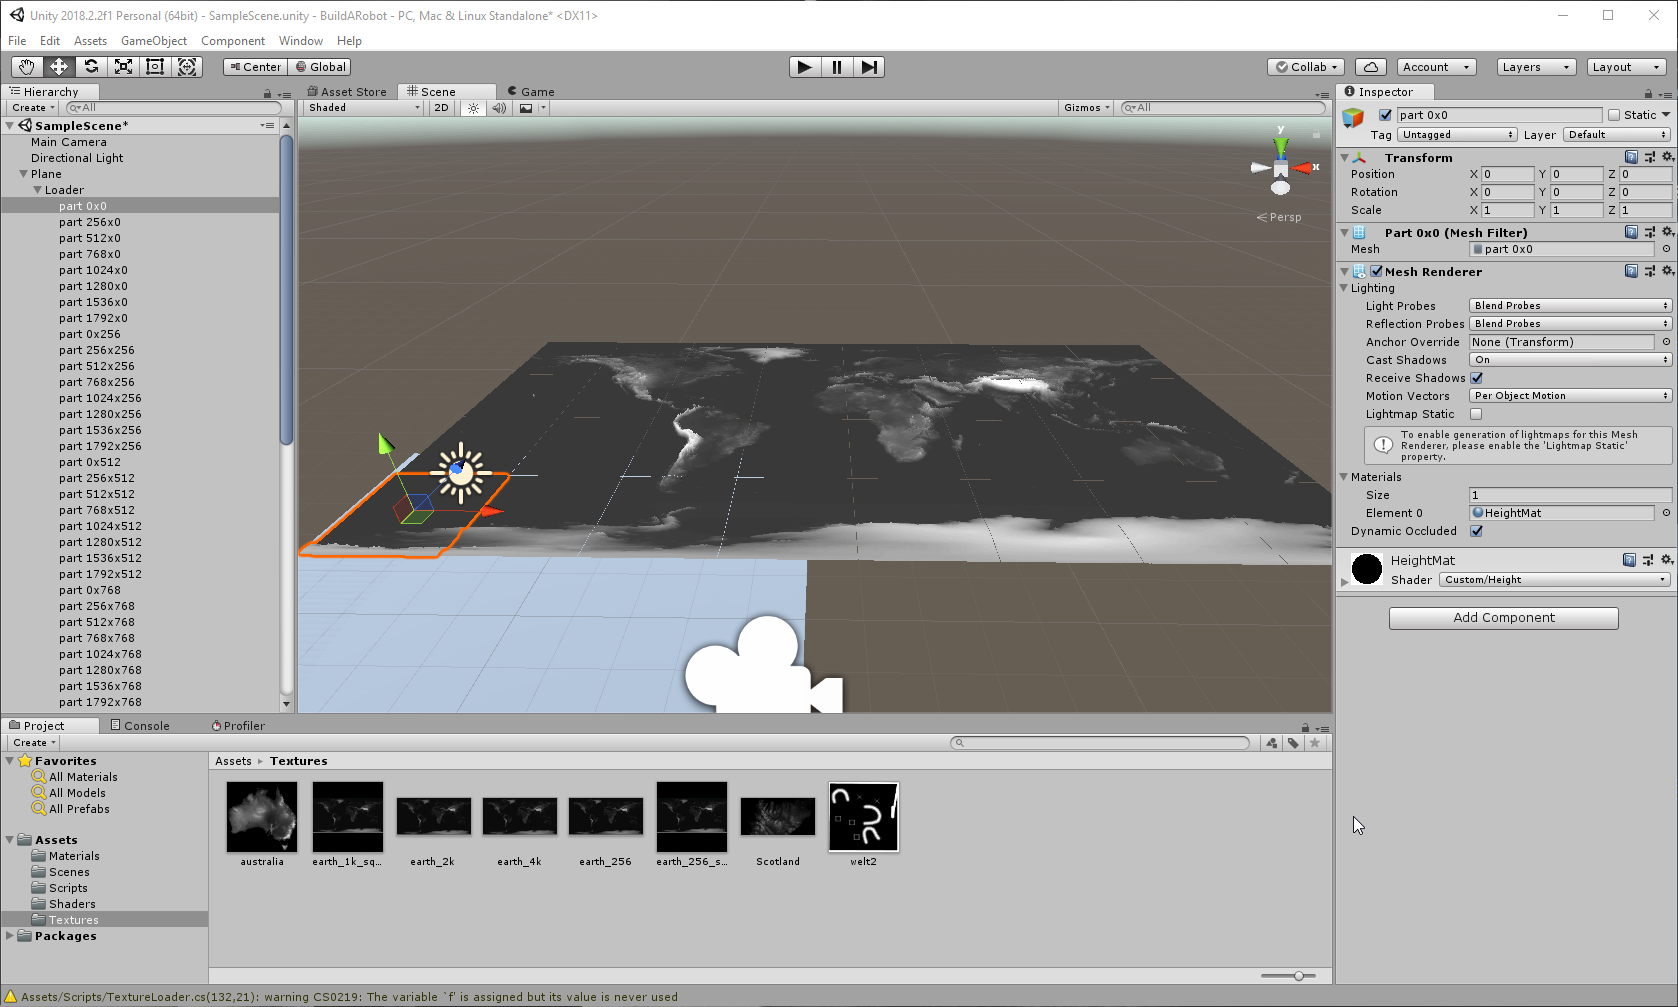
\includegraphics[width=14cm]{tex/img/ch05/UnityScreenshot.png}
\captionof{figure}{The Unity Editor}
\label{fig:unity-editor}
\end{center}

%////////////////////////////////////////////////
\subsection{Designer: Building the Scene}
\subsubsection{Rebuilding a real environment}
As stated in \ref{section:goals-and-constraints} the environment used to base a scene on was the second floor of building "A" of University of Applied Sciences Mannheim. However at this time no 3D model of the floor, let alone the building existed so it had to be handcrafted using the resources that were available: a floor plan (shown in Figure \ref{fig:floor-plan-image}) and measurements taken by hand.
% tex/img/ch05/FloorPlan03_small.JPG
% \label{fig:floor-plan-image}
% tex/img/ch05/BlenderFloor01.png
% \label{fig:floor-plan-blender}
\newlength{\twosubht}
\newsavebox{\twosubbox}

\begin{figure}[htp]
    % preliminary
    \sbox\twosubbox{%
      \resizebox{\dimexpr.9\textwidth-1em}{!}{%
        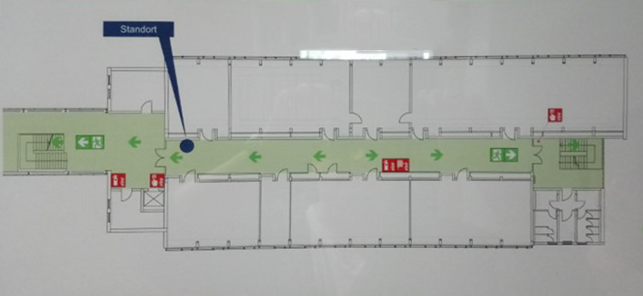
\includegraphics[height=3cm]{tex/img/ch05/FloorPlan03_small.JPG}%
        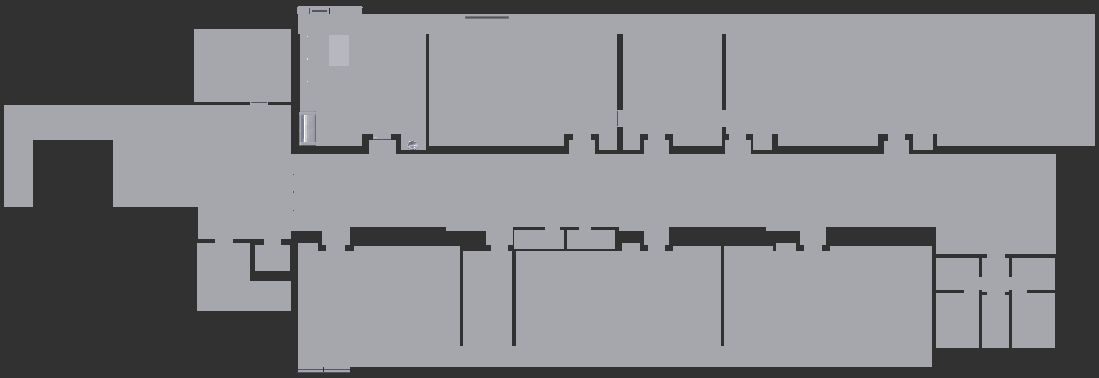
\includegraphics[height=3cm]{tex/img/ch05/BlenderFloor01.png}%
      }%
    }
    \setlength{\twosubht}{\ht\twosubbox}
    % typeset
    \centering
    \subcaptionbox{\label{fig:floor-plan-image}}{%
      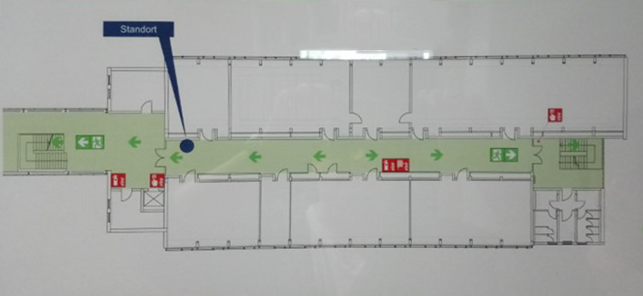
\includegraphics[height=\twosubht]{tex/img/ch05/FloorPlan03_small.JPG}%
    }\quad
    \subcaptionbox{\label{fig:floor-plan-blender}}{%
      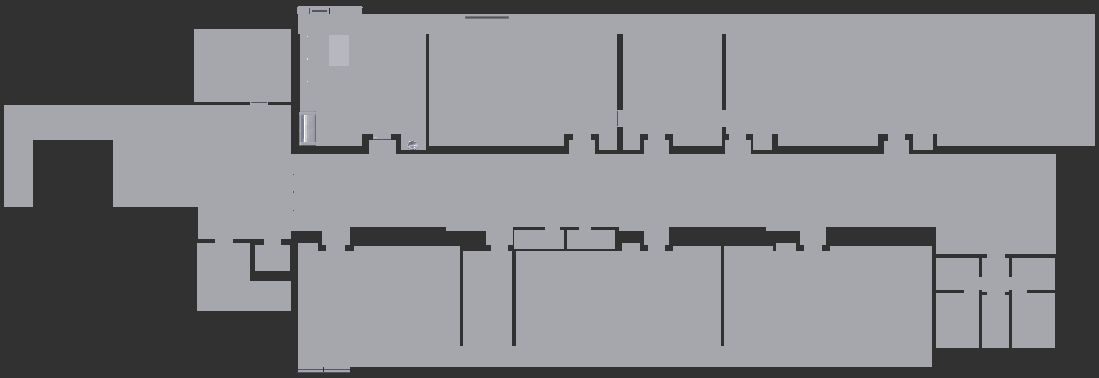
\includegraphics[height=\twosubht]{tex/img/ch05/BlenderFloor01.png}%
    }
    \caption{Floor plan, photo (\ref{fig:floor-plan-image}) and reconstruction in Blender (\ref{fig:floor-plan-blender})}
\end{figure}

Figure \ref{fig:floor-plan-blender} shows the reconstruction of the basic layout of the floor in Blender. As the goal of this implementation was to generate records used for detecting doors, special attention had to be paid to modeling the doors in this floor. This required taking measures of the doors themselves, their handles and frames as well as reconstruction of the properties of their surfaces. Figure \ref{fig:doors} shows the various doors present on this floor: utility doors (shown in \ref{fig:door01} featured metallic handles, a black and matte metal surface and were broader than most other doors. Lecture doors (\ref{fig:door02}) had blue matte metal surfaces and were not on the same level as the walls but inset into the walls. They also had glass-panels located right above them. The portals (\ref{fig:door03}) to the lecture rooms, one present at each end of the hallway, had glass doors and panels and matte black metal beams and frames. Lastly there were doors to storage rooms (\ref{fig:door04}) that did not feature great geometrical detail as the other doors did. They blended into the wall and featured shiny metal knobs and hinges.
%Fokus: Türen, möglicherweise Hindernisse im Weg (Stühle), interessant waren Fenster, im FLur nur indirekt Beleuchtung, Wände (Reflektionen, Helligkeiten), verschiedene Türen (Overfläche, Farbe, Geometrie [Glas, Fenster, Mauer])

\begin{figure}[htp]
    % preliminary
    \sbox\twosubbox{%
      \resizebox{12cm}{!}{%
        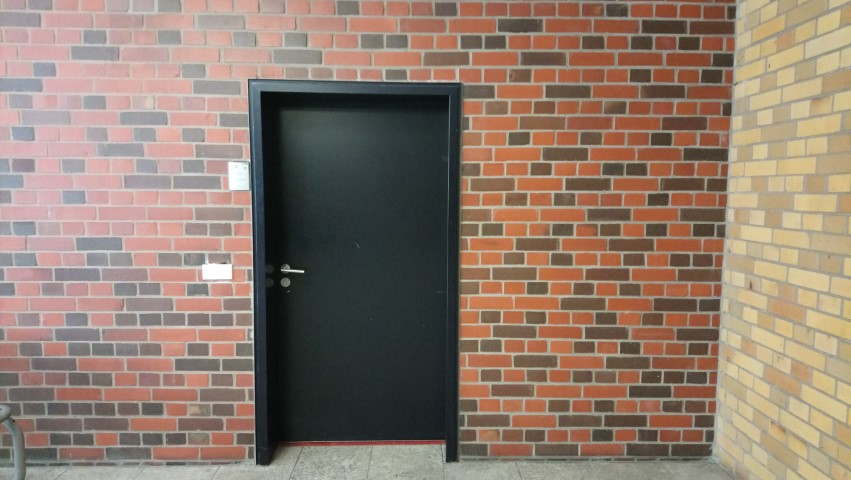
\includegraphics[height=6cm]{tex/img/ch05/Door01_small.JPG}%
        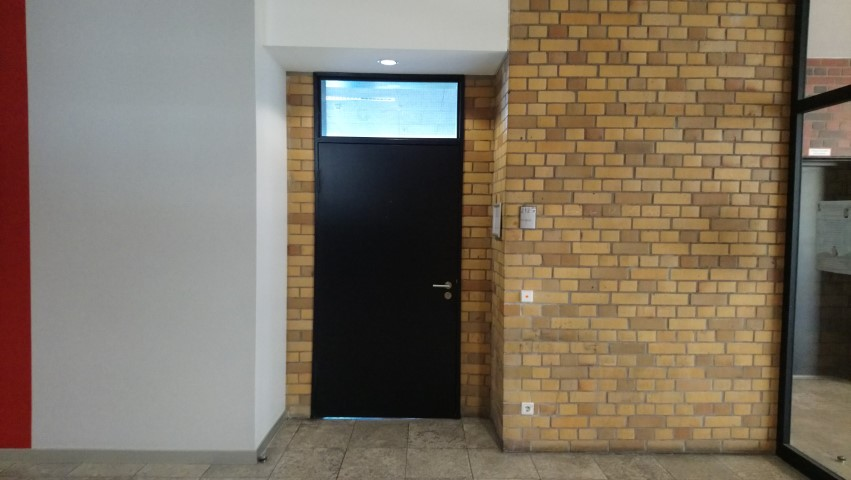
\includegraphics[height=6cm]{tex/img/ch05/Door02_small.JPG}%
        %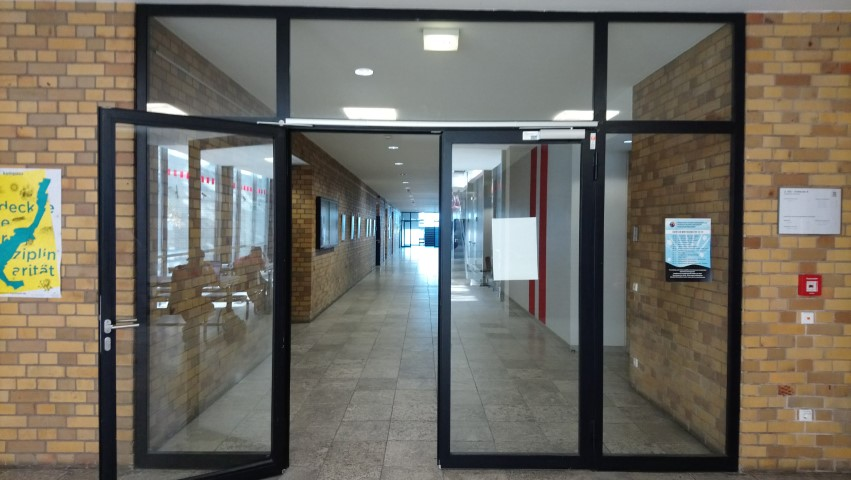
\includegraphics[height=6cm]{tex/img/ch05/Door04_small.JPG}%
        %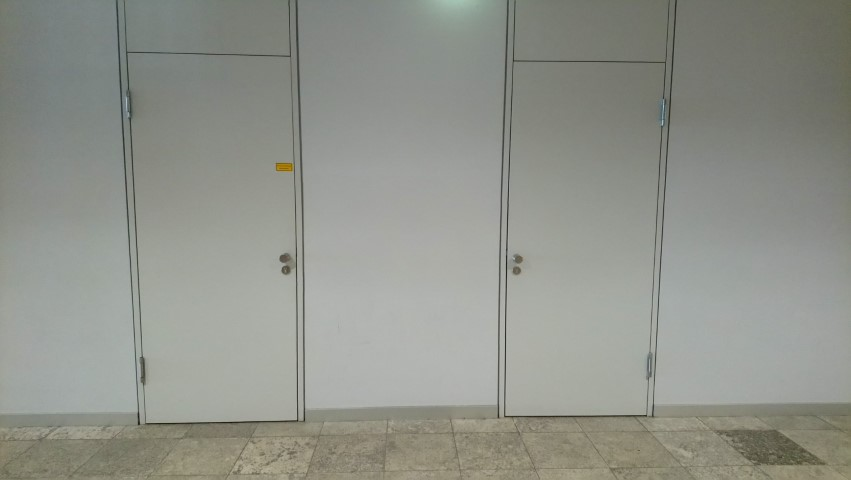
\includegraphics[height=6cm]{tex/img/ch05/Door05_small.JPG}%
      }%
    }
    \setlength{\twosubht}{\ht\twosubbox}
    % typeset
    \centering
    \subcaptionbox{\label{fig:door01}}{%
      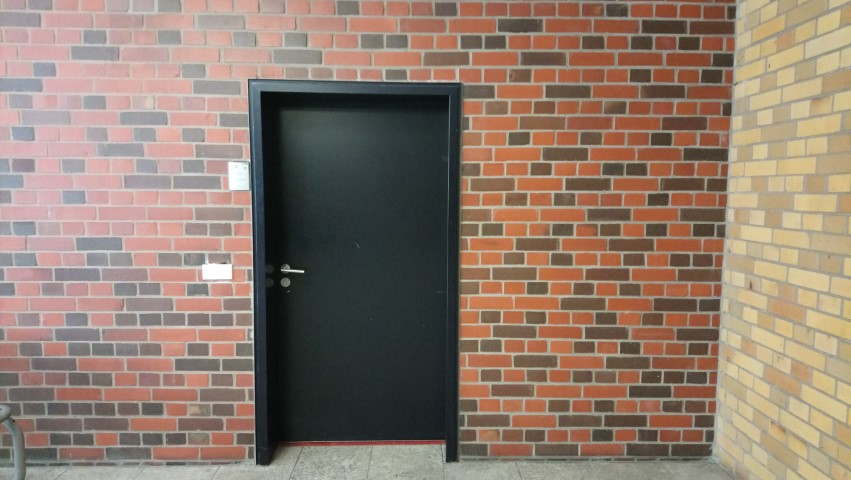
\includegraphics[height=\twosubht]{tex/img/ch05/Door01_small.JPG}%
    }\quad
    \subcaptionbox{\label{fig:door02}}{%
      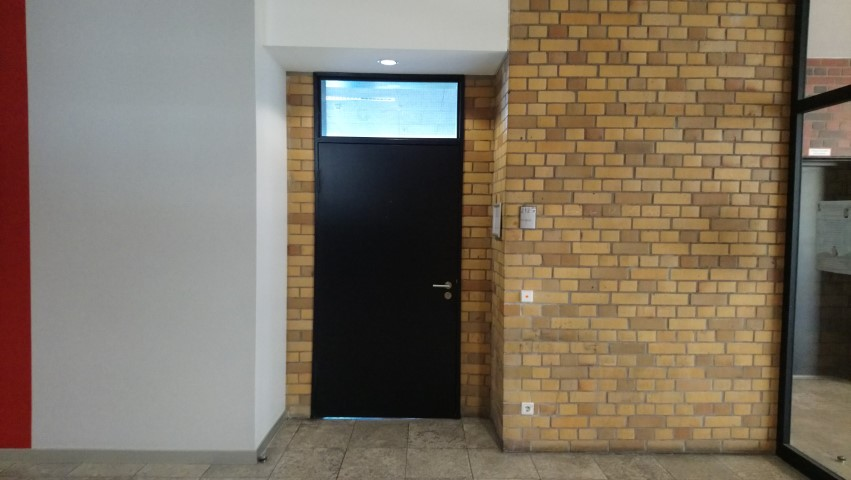
\includegraphics[height=\twosubht]{tex/img/ch05/Door02_small.JPG}%
    }\\%quad
    \subcaptionbox{\label{fig:door03}}{%
      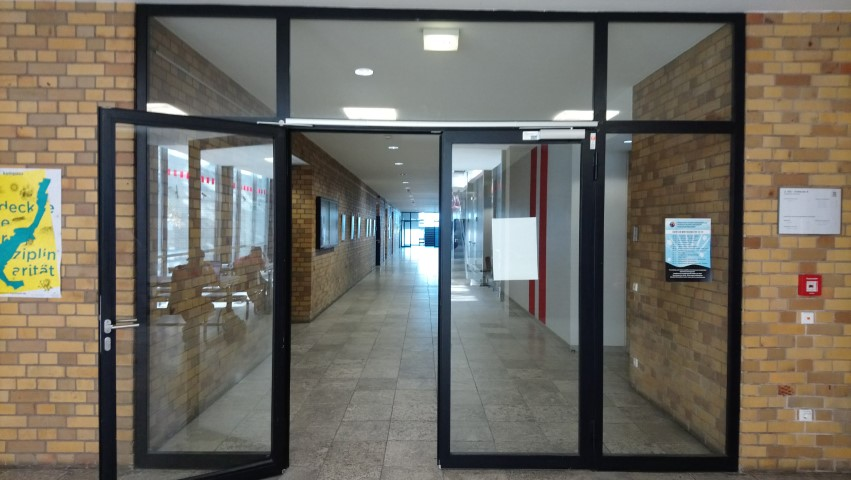
\includegraphics[height=\twosubht]{tex/img/ch05/Door04_small.JPG}%
    }\quad
    \subcaptionbox{\label{fig:door04}}{%
      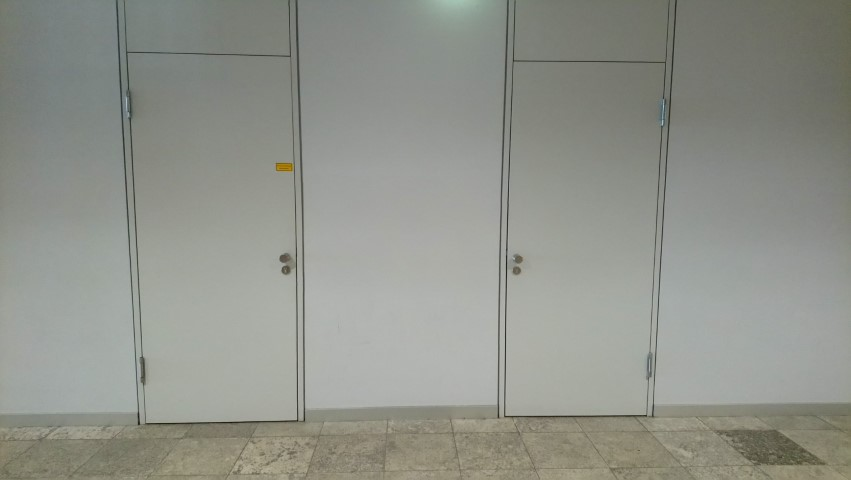
\includegraphics[height=\twosubht]{tex/img/ch05/Door05_small.JPG}%
    }
    \caption{Various different doors on the floor}
    \label{fig:doors}
\end{figure}

The reconstructed doors could now be used to render very detailed door meshes with realistic surfaces. However other objects had to be reconstructed: as lighting would have great influence on the generated images, the large window facades covering the building and feature blinds were added to the scene along with a set of other common objects present in the floor like air-conditioning pipes on ceiling, radiators and tables. Figure \ref{fig:unity-scene-a205} shows the final reconstruction of the room A205 which is the first room on the second floor. It features windows with blinds that cast shadows on the walls and objects and it features obstacles (such as tables) that may occlude other objects of interest such as the doors.

\begin{center}
\noindent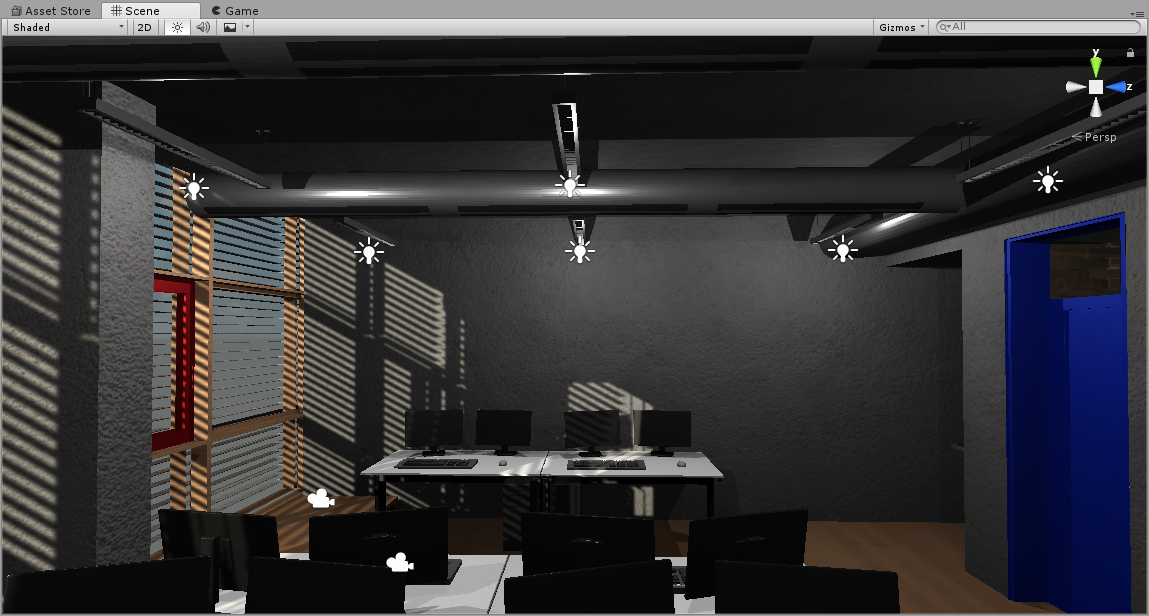
\includegraphics[width=14cm]{tex/img/ch05/UnitySceneA205_02.png}
\captionof{figure}{Reconstruction of room A205 in Unity Editor}
\label{fig:unity-scene-a205}
\end{center}

\subsection{Importing Robots into Scenes}
After recreation of the scene's geometry, a robot was needed for \acp{AI} engineers to navigate around the scene and capture records. For this implementation the robot model "Pioneer 3AT" was chosen as the Institute of Robotics of University of Applied Sciences Mannheim works with "Pioneer"-robots and there were \acp{URDF} files of it available \cite{AmrRosConfig} online.\\
There were few libraries that provide methods to import robots using URDF-files into Unity, an extensive one was \textit{"ROS\#"} which was developed by Siemens AG. It was described as "a set of open source software libraries and tools in C# for communicating with ROS from .NET applications, in particular Unity3D" \cite{RosSharp}. This project implemented connecting to ROS instances, ROS' publish/subscribe pattern and importing robots into Unity scenes, however its software design introduced some potential problems: 
\begin{enumerate}
    \item Importing robots using URDF-files was done by downloading URDF-files from running ROS-instances. The need for a running ROS-instance would add to the system requirements VERE runs on.
    %ros-sharp/Unity3D/Assets/RosSharp/Scripts/Urdf/Editor/UrdfComponents/UrdfRobotExtensions.cs
    \item ROS\#'s URDF importing component required the URDF files to be present in the "Asset" folder of Unity-projects. This meant that URDF-files downloaded from remote locations needed to be written to disk and compressed archives that contained additional files like meshes and textures needed to be extracted to disk first.
    \item Even though robots imported by ROS\# had the correct hierarchy of body-parts and correct physical properties (as defined in the robots' URDF), Unity's physics engine often times failed to simulate physics wrong at run-time, leading to robots being unable to move, falling through floors or being propelled into the air.
\end{enumerate}

To solve the first two problems, a simple set of filesystem-interfaces (were implemented fpr local filesystems and ZIP-archives.

\begin{center}
\noindent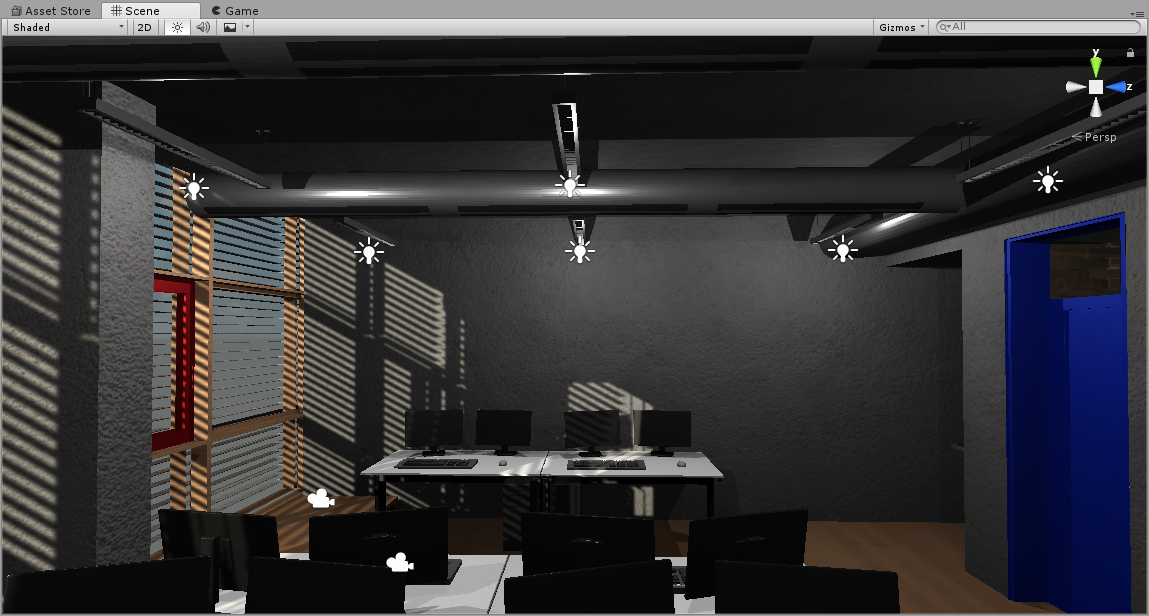
\includegraphics[width=14cm]{tex/img/ch05/UnitySceneA205_02.png}
\captionof{figure}{Reconstruction of room A205 in Unity Editor}
\label{fig:unity-scene-a205}
\end{center}

\subsection{Identifying Classifiers}
% ** WorldToScreen
\subsubsection{Approach I: Using Coordinate-Transformations}
WorldToScreen (Bounding boxes/Colliders) [TBD]

% ** Raycasting
\subsubsection{Approach II: Raycasting}
[TBD]

%////////////////////////////////////////////////
\subsection{AI Engineer: Capture Records}
\subsubsection{Controlling the Robot}

\subsubsection{Controlling the Robot}

%////////////////////////////////////////////////
\subsection{Results}

%////////////////////////////////////////////////
\section{Implementation II: Using Blender as an Offline Renderer}
Goal: Use Blender as an offline renderer, allowing for potentially photorealistic images being generated using a raycasting engine like cycles.

%////////////////////////////////////////////////

